%%==================================================
%% chapter03.tex for TJU Master Thesis
%% Encoding: UTF-8
%%==================================================

\chapter{编织层准静态强度及内压爆破实验仿真}


\section{引言}

前面一章针对编层的非线性力学行为,进行了理论体系的修正和拓展,取得了较好的效果,本章则是对该理论模型在内压荷载的应用。
首先,本章要明确该理论体系如何确定特征单元的应力应变状态与编织层纤维应力应变状态,这实际上是与前一章中“平均化”相反的过程。
其次,本章要明确如何将理论结果应用到内压爆破试验中去。因为内压爆破试验是一个动态加载的过程,而前一章中得到的理论体系实际上是在准静态的条件下得到的。

\section{准静态强度判定}

编织层特征单元的应力应变状态可以通过特征单元的几何关系推导出编织层纤维的伸长量。而纤维本身的额定破坏应力的大小决定了纤维的最大伸长率。可以以此作为判断编织层是否发生破坏的准则:

\begin{equation}
{\sigma _f} = {\varepsilon _f} \cdot E \le \left[ {{\sigma _u}} \right]
\end{equation}

根据特征单元的几何关系,如图\ref{fig:unit-cell-chap6}所示,编织层纤维的纤维向应变$  \sigma _f$为:


\begin{figure*}[!htb]
	\centering
	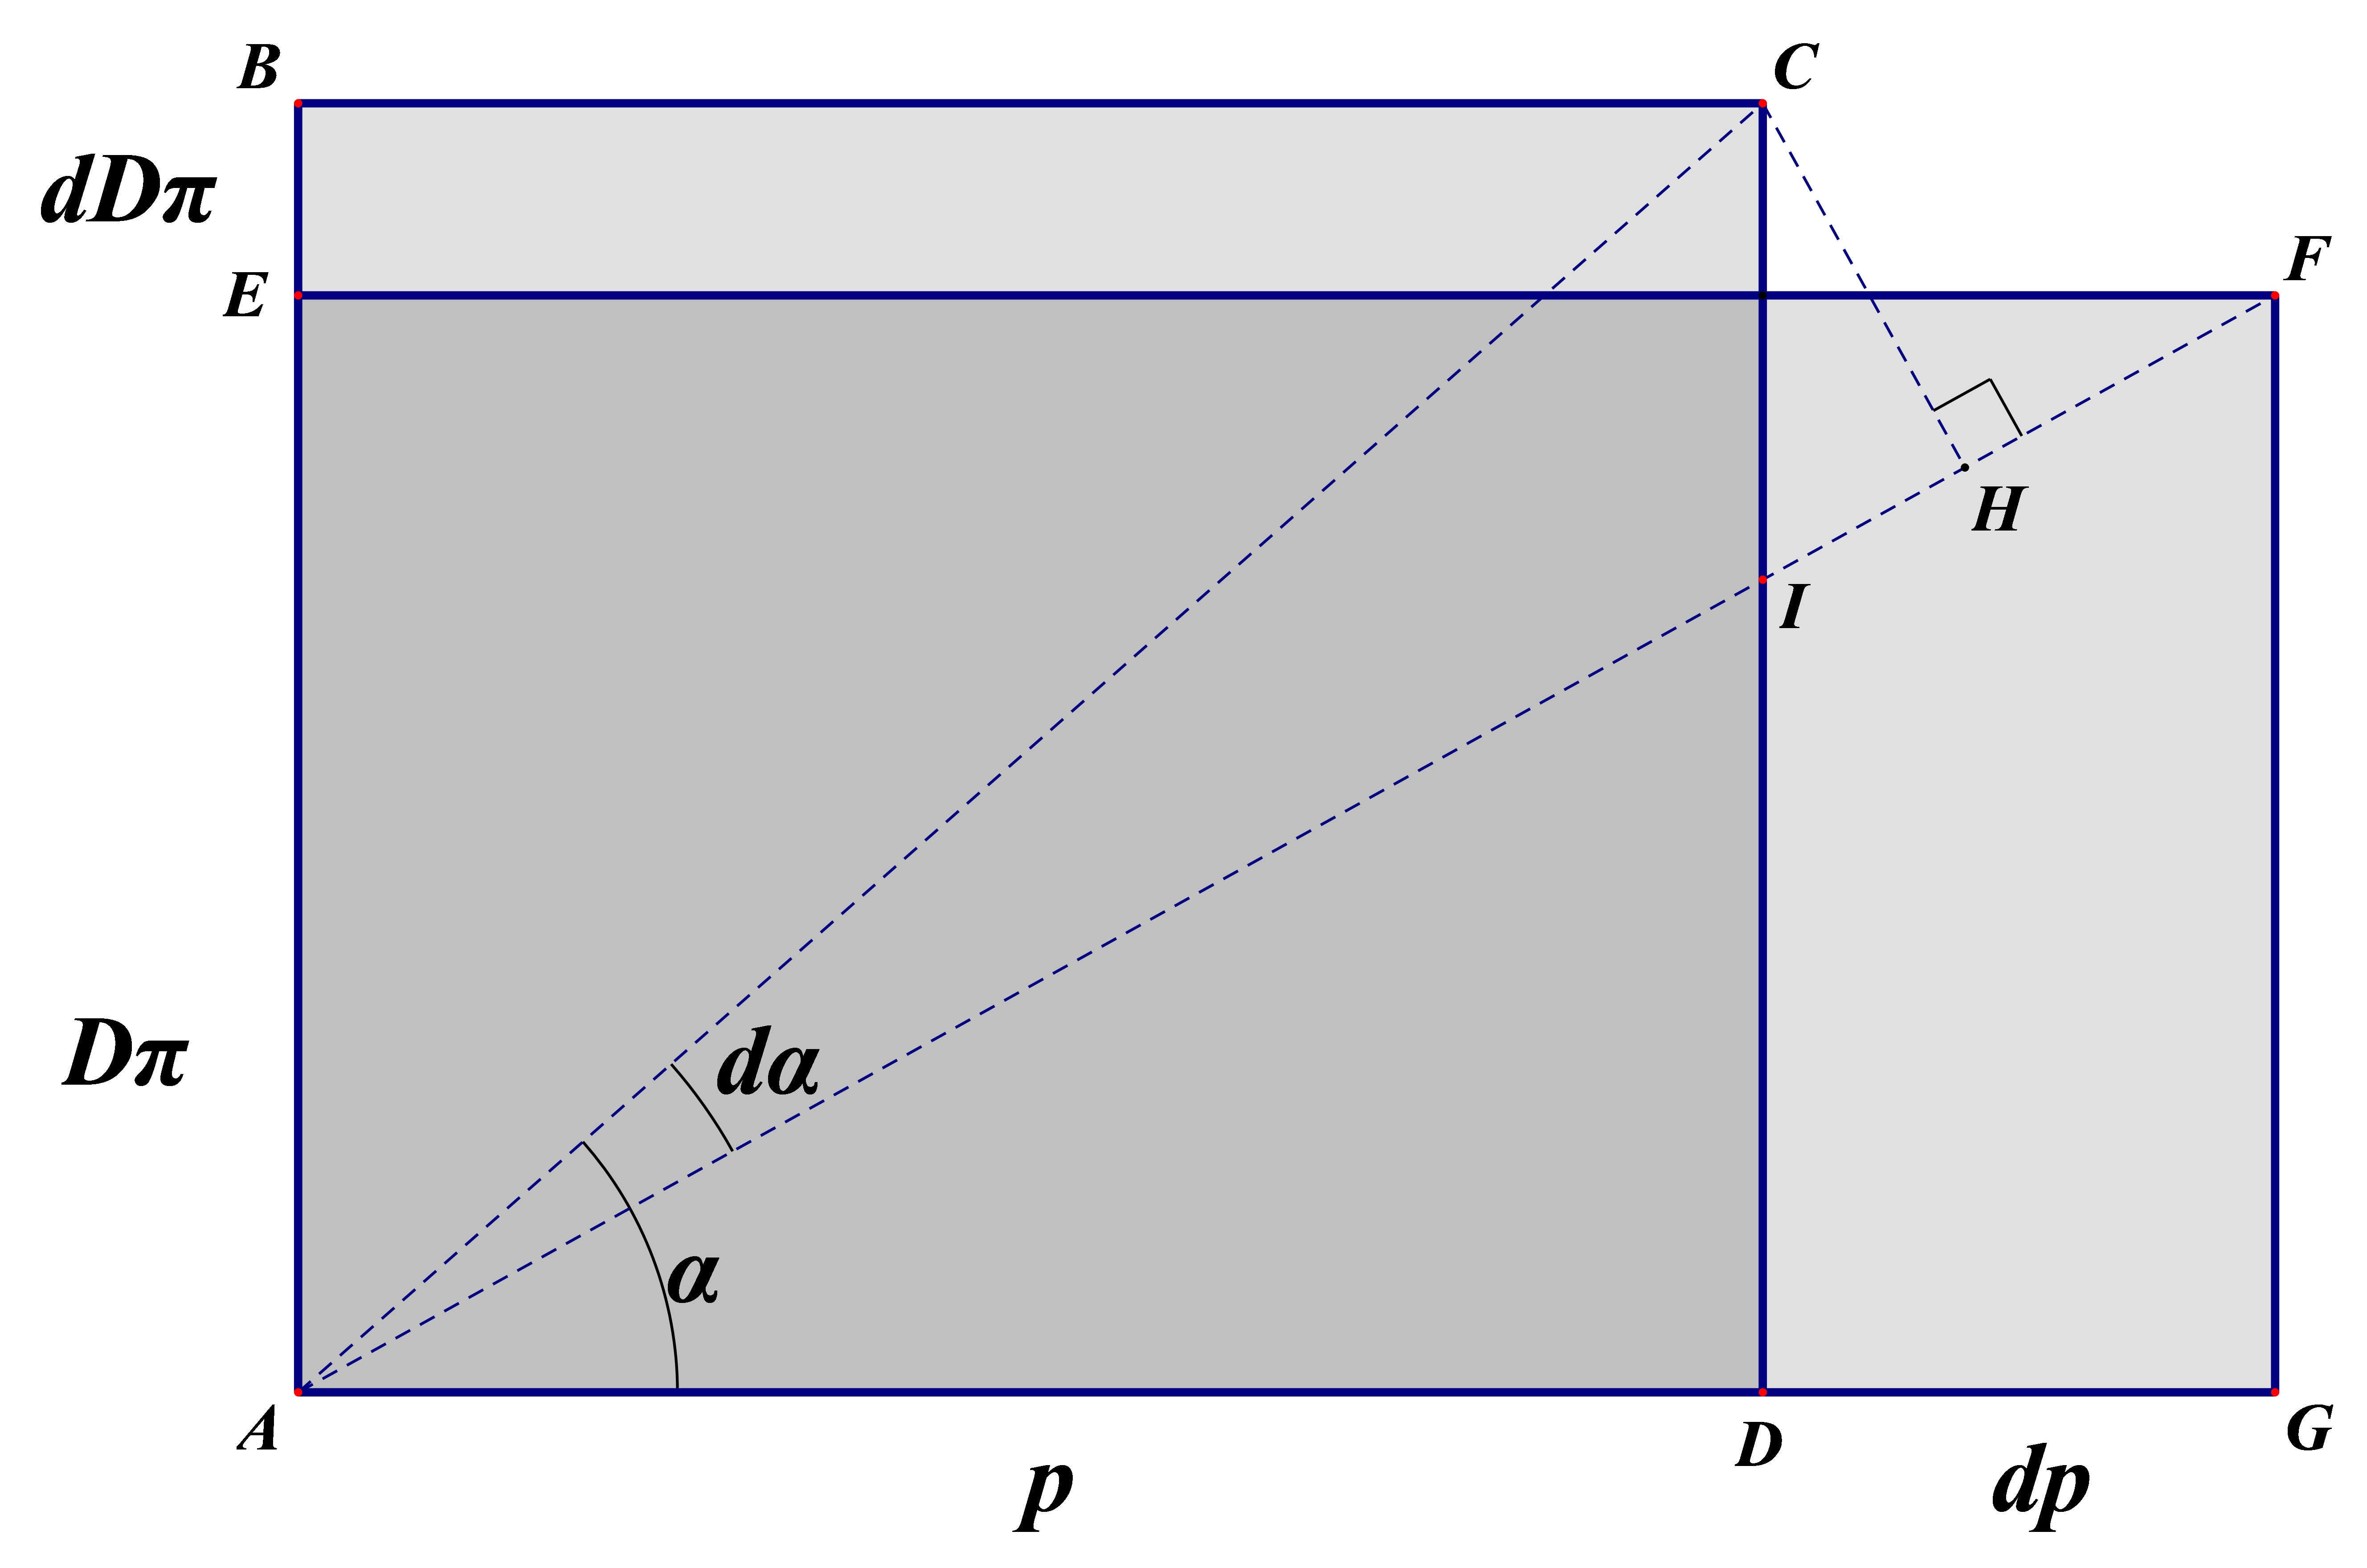
\includegraphics[height=0.25\textheight]{figure/chap5/unit-cell-3}
	\fcaption{特征单元的纤维方向伸长}{elongation of the representative unit cell in fiber direction}
	\label{fig:unit-cell-chap6}
\end{figure*}


\begin{equation}
\label{eq:fiber-elongation}
{\varepsilon _f} = \sqrt {\frac{{{{\left( {{\varepsilon _{22}} + 1} \right)}^2} + \tan {\alpha ^2}{{\left( {1 - {\varepsilon _{33}}} \right)}^2}}}{{1 + \tan {\alpha ^2}}}}  - 1
\end{equation}



\subsection{拉伸实验仿真结果对比}

对比数值模拟的拉伸实验仿真结果,接头颈缩处为纤维伸长量最大处(图\ref{fig:strength}云图中红色区域)与实验结果吻合,应力大小为2000MPa ;金属纤维的额定模量也为2000MPa。可以认为该理论对于准静态的加载状态有效。

\begin{figure*}[!htb]
\centering
\emph{}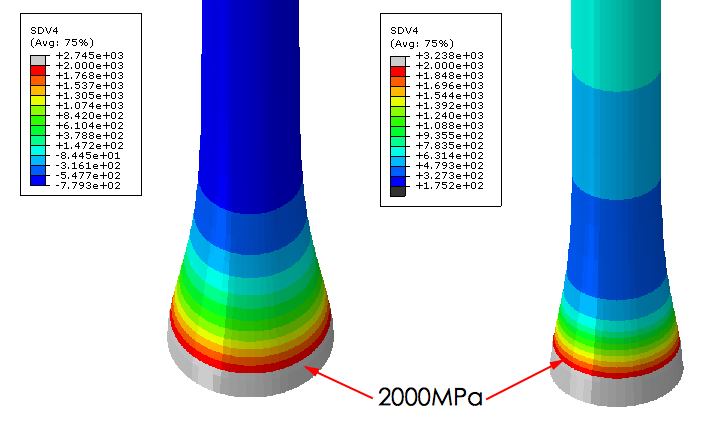
\includegraphics[height=0.25\textheight]{figure/chap6/strength}
\fcaption{修正模型仿真拉伸实验纤维应力分布云图}{stress in fiber direction with modified model}
\label{fig:strength}
\end{figure*}

\ha 基本理论事实上并没有考虑编织层强度的算法,但根据其特征单元同样可以求出纤维也可以推得的纤维向应变 ,

\[{\varepsilon _f} = \sqrt {\frac{{{{\left( {{\varepsilon _{22}} + 1} \right)}^2} + \tan {\alpha ^2}}}{{1 + \tan {\alpha ^2}}}}  - 1\]

\begin{equation}
= \cos \left( {\alpha  - d\alpha } \right)\cos \alpha  \cdot {\varepsilon _{22}} - \frac{{{{\left( {d\alpha } \right)}^2}}}{2}
\end{equation}

上式基于未修正的特征单元几何模型,在特征单元的层面上,并没有考虑管径变化对纤维应变的影响。而从钢绞线理论出发,研究发现是很难回归到纤维方向的应变上的。
利用该式得到的纤维向应力云图\ref{fig:hose-strength002}, 
并不能得到正确的应力分布,发生断裂的接头处纤维的反而是应力最小处,显然不能将该理论应用于编织层的设计。
\begin{figure*}[!htp]
	\centering
	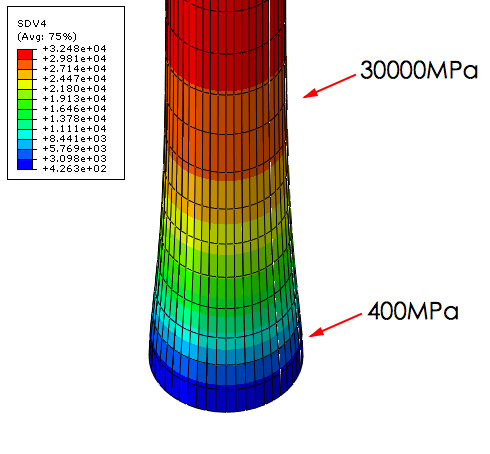
\includegraphics[height=0.26\textheight]{figure/chap6/hose-strength002}
	\fcaption{未修正拉伸试验纤维应力分布}{ stress in fiber direction with Hachemi's model}
	\label{fig:hose-strength002}
\end{figure*}

 






\section{内压爆破强度判定}

由于内压爆破实验的加载过程升压速率非常快,约为30MPa/s\footnote{SAE AS1946},不能视为准静态过程。但是该过程的振动、激励不是研究的重要对象,仅仅需要研究金属纤维最终是否会断裂。因此这里通过材料力学中的突加荷载的方法:根据达朗贝尔原理,一个动荷载,可以利用准静态的计算结果$ \sigma $与动荷载系数$ K $相乘得到动荷载下的状态。

由于爆破内压加载速度极快,可以视为突加荷载。突加荷载的系数$ K=2 $,乘以准静态结果,
就可以得到爆破内压实验荷载下编织层纤维的应力应变状态。



\begin{equation}
K\cdot\sigma _{static}=2\sigma _{static}= \sigma _{burst}
\end{equation}

 相当于将准静态时的强度极限折减到原来的二分之一。
 满足式\ref{eq:st-lim}就可以认为纤维尚未发生断裂,该压力下软管组件安全。$ {\sigma _f^{static}} $为准静态分析中纤维上的应力。
 
\begin{equation}
\label{eq:st-lim}
{\sigma _f^{static}}  \le \frac{1}{K} \left[ {{\sigma _u}} \right] = \frac{1}{2} \left[ {{\sigma _u}} \right]
\end{equation}


根据该理论,减小升压速率,$ K $值就会减小,相应的爆破压力值应该会上升。实际上,降低升压速率,相同编织层可以达到的爆破压力值会减小,因为,此时初始缺陷等因素的影响就开始占据主导地位。


\subsection{内压爆破仿真}

进行内压实验的有限元仿真,同样采用\uma 导入本文的理论模型。首先根据确定的软管组件的规格进行完整的几何建模,然后逐步开始施加内压荷载。当发现纤维方向的应变$ \varepsilon_f $达到极限应力对应的应变的二分之一时,停止增加内压荷载,此时内压荷载的大小就是该规格软管组件的爆破压力值。图\ref{fig:chap6-hose-burst}为不同规格软管组件受内压荷载是的状态。



本文首先对Φ5(10.5MPa)软管组件进行了内压爆破的仿真\footnote{内压爆破实验数据由上海市塑料研究所提供},验证修正非线性段软管组件的本构修正对内压爆破荷载仿真效果的影响。因其经过拉伸实验验证,可以对比拉伸力位移曲线的拟合程度对爆破压力仿真值的影响。仿真结果的纤维向应力值由式\ref{eq:fiber-elongation}求得。


\begin{table}[!htbp]
	\centering
	\tcaption{ Φ5(10.5MPa)软管组件内压模型修正效果}{Φ5(10.5MPa)hose modified FEM results contrast}
	\label{tab:strength-of-hose-results}
	\begin{tabular}{@{\extracolsep{\fill}}>{\hspace{0.5cm}}clcccc}
		\toprule
		&平面内纤维&斜穿纤维&加速系数&爆破压力&相对误差\\\midrule
		修正-1&0.5&0.5&1.15&96.7MPa&0.31\%\\
		修正-2&0.5&0.5&1&94.9MPa&-1.56\%\\
		未修正&1&0&1&84.5MPa&-12.34\%\\
		\bottomrule
	\end{tabular} 
\end{table}  


表\ref{tab:strength-of-hose-results}给出了不同修正参数求得的爆压力值,而各组修正参数对应的拉伸力位移曲线如图\ref{fig:strength-elongation}所示。


\begin{figure*}[!htp]
	\centering
	\subfigure[不同修正参数软管拉伸力位移曲线]{
		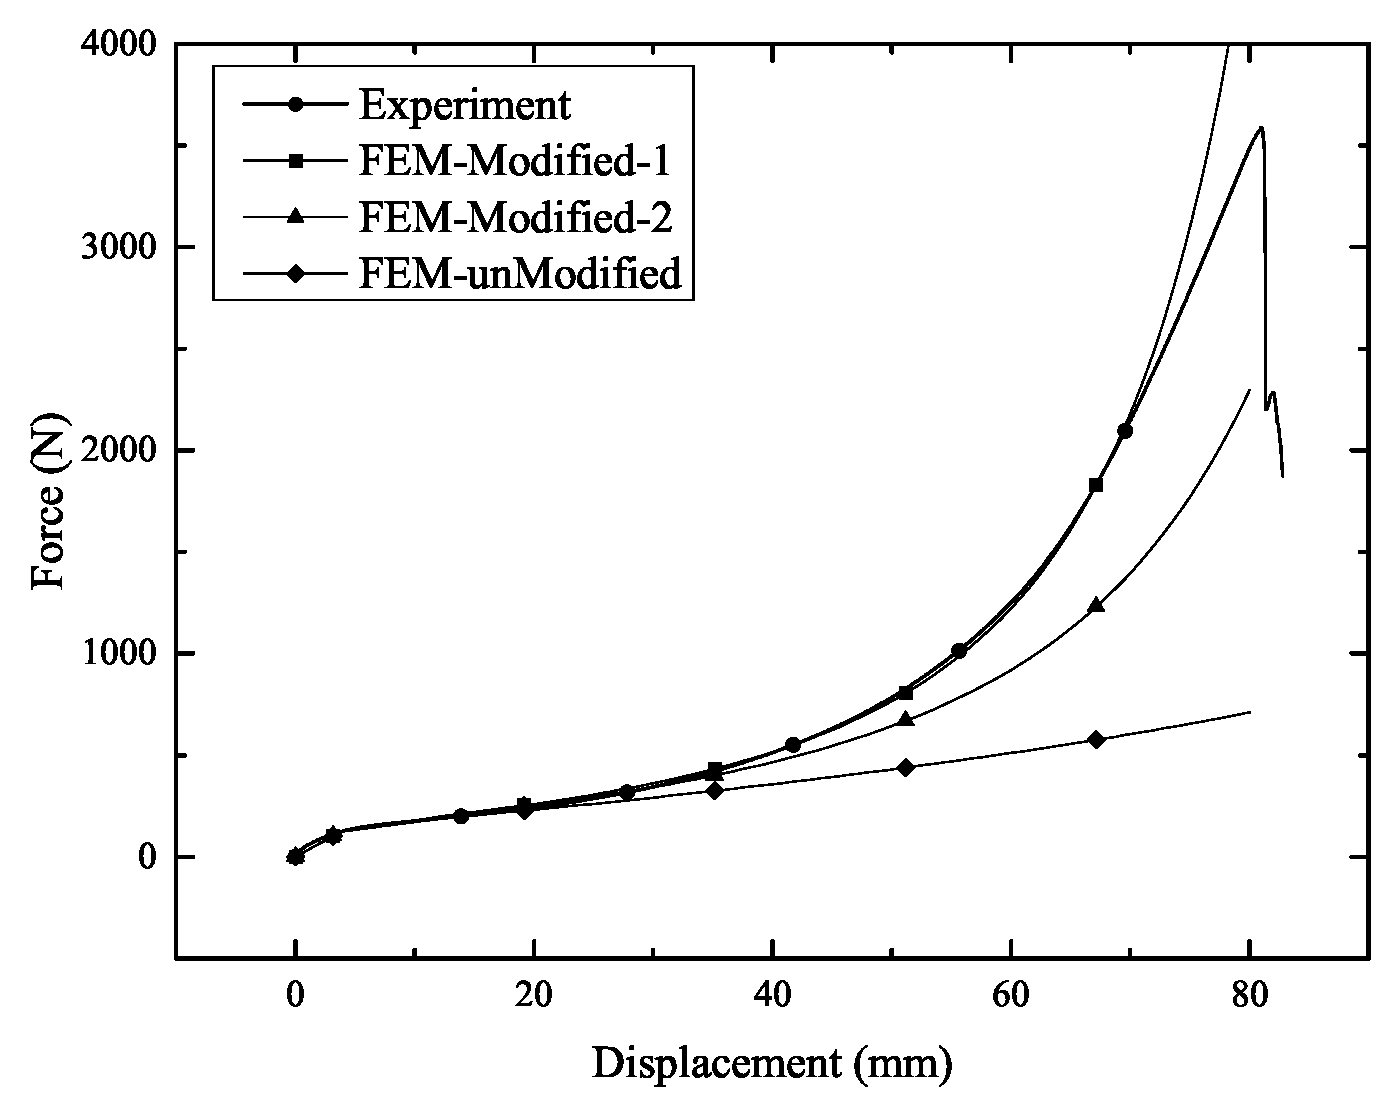
\includegraphics[width=0.5\linewidth]{figure/chap6/Graph152}	
		\label{fig:strength-elongation}
	}
	\hspace{0.5cm}
	\subfigure[软管受内压荷载变形]{
		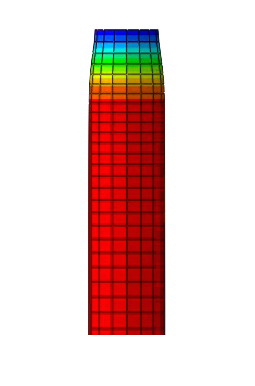
\includegraphics[width=0.25\linewidth]{figure/chap6/stress}
	}
	\fcaption{内压爆破试验仿真效果}{burst pressure simulation results}
	\label{fig:stress}
\end{figure*}


根据表\ref{tab:strength-of-hose-results}给出的仿真结果,可以发现,\ha 理论计算的爆破压力值,对比修正模型,误差较大。
分析认为:\ha 理论在只在线性段拟合的比较好,而内压爆破荷载下软管的变形,大部分发生在线性段,小部分发生在非线性段,并不像拉伸实验那么明显,因而\ha 未修正的仿真结果大致正确 。








\begin{table}[!htb]
	\centering
	\tcaption{ 不同规格软管组件实验及有限元爆破压力}{exprimental and FEM caculated burst pressure of hoses}
	\label{tab:strength-of-hose}
	\begin{tabular}{@{\extracolsep{\fill}}>{\hspace{0.5cm}}clcccc}
		\toprule
		序号 &    规格     & \tabincell{c}{编织形式\\/mm×根 }& \tabincell{c}{实际\\爆破值/MPa }& \tabincell{c}{计算\\爆破值/MPa}& \tabincell{c}{偏差\\百分比}  \\ \midrule
		1  & Φ5(10.5MPa)  & Φ0.2×6  &   96.4    & 96.7          & 0.31\% \\
		2  & Φ8(10.5MPa)  & Φ0.3×5  &   83.5    & 83          & -0.60\% \\
		3  & Φ12(10.5MPa) & Φ0.3×6  &   63.5    & 66          & 3.94\%  \\
		4  & Φ16(5.0MPa)  & Φ0.3×6  &   47.1    & 51          & 8.28\% \\ \bottomrule
	\end{tabular} 
	\end{table}  

修正后的理论模型可以考虑非线性段的影响,仿真求得的爆破压力值更接近大量实验的统计值。对不同规格的软管组件采用$ V_w=0.5,V_s=0.5,k=1.0 $的修正参数对编制层的刚度进行修正。仿真爆破压力值如表\ref{tab:strength-of-hose}所示。

\begin{figure*}[!htp]
	\centering
	
	\subfigure[]{
		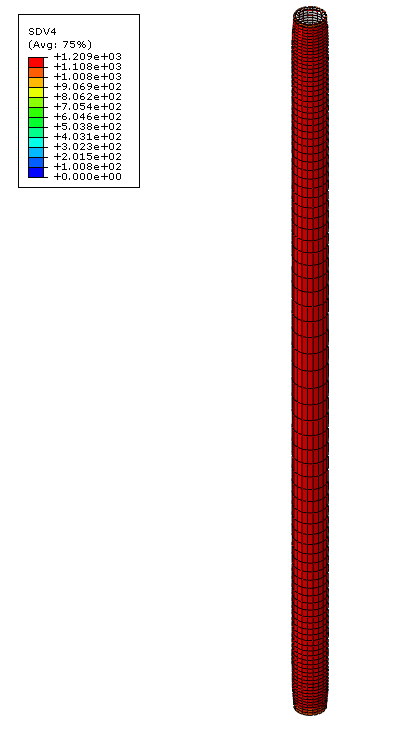
\includegraphics[height=0.33\textheight]{figure/chap6/1}
		\label{fig:chap6-1}
	}
	\subfigure[]{
		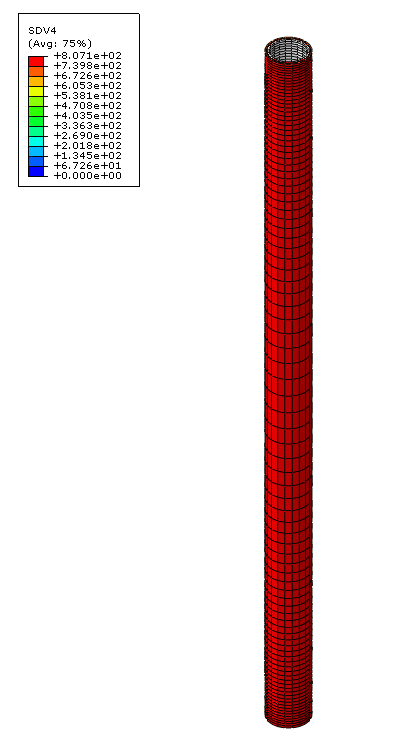
\includegraphics[height=0.33\textheight]{figure/chap6/2}
		\label{fig:chap6-2}
	}
	\fcaption{不同规格软管组件内压爆破实验仿真}{deformation of hose under burst pressure with modified model}
	\label{fig:chap6-hose-burst}
\end{figure*}


几组软管的爆破压力值计算误差都均在$ 10\% $以内,可以认为该算法稳定有效。


\section{小 ~ 结}

本章主要利用前文修正的纤维编织层本构模型,对内压爆破实验进行了仿真,对比了爆破实验的数据,验证了通过拉伸实验修正的理论可以应用与不同工况的仿真。

在进行内压爆破的仿真之前,本章推导了修正理论模型在纤维方向上的应变的计算方法,对拉伸实验进行了强度的验证。

然后,本章利用材料力学突加荷载理论,利用准静态的仿真,等效模拟内压爆破荷载的工况,并提出了强度换算的方法。
